%%%%%%%%%%%%%%%%%%%%%%%%%%%%%%%%%%%%%%%%%%%%%%%%%%%
% DOCUMENT CLASS DECLARATION
%%%%%%%%%%%%%%%%%%%%%%%%%%%%%%%%%%%%%%%%%%%%%%%%%%%
%% Use the following options:
% \documentclass[paper type% ("letterpaper" required)
% , one or two sided% ("oneside" or "twoside")%
% , font size% ("12pt" required)%
% , document type% ("these", "memoire", "memoirepararticles", "memoireprojet" or "thesepararticles")%
% , document language ("francais" or "english)%
% , addition options% ("creativecommons" if the document is under the creative commons license, "hyperref", "withAlgo2e" to use algorithm2e package with proper formating)
%]{thETS}

%% Exemple with a Ph.D thesis under creative commons, using hyperref
\documentclass[letterpaper%
, oneside%
, 12pt%
,thesepararticles%
, english%
,creativecommons,hyperref, withAlgo2e%
]{thETS}

%%%%%%%%%%%%%%%%%%%%%%%%%%%%%%%%%%%%%%%%%%%%%%%%%%%
% IMPORTANT: PRINTING WITH THE PROPER MARGINS
%%%%%%%%%%%%%%%%%%%%%%%%%%%%%%%%%%%%%%%%%%%%%%%%%%%
%% Always set the "scaling" option to "none" in the prining options 
%% to print the generated PDF with the proper margins.
%%%%%%%%%%%%%%%%%%%%%%%%%%%%%%%%%%%%%%%%%%%%%%%%%%%


%%%%%%%%%%%%%%%%%%%%%%%%%%%%%%%%%%%%%%%%%%%%%%%%%%%
% DECLARATION OF AN ADDITION LIST OF REFERENCES
%%%%%%%%%%%%%%%%%%%%%%%%%%%%%%%%%%%%%%%%%%%%%%%%%%%
%% Exemple of an additional list of references called "refs"
% "refs" is used as a suffix to all bibliography related commands
\newcites{refs}{LIST OF REFERENCES}

%%%%%%%%%%%%%%%%%%%%%%%%%%%%%%%%%%%%%%%%%%%%%%%%%%%
% TITLE PAGE OPTIONS
%%%%%%%%%%%%%%%%%%%%%%%%%%%%%%%%%%%%%%%%%%%%%%%%%%%

\title{Adaptive Collaborative Autonomous Wireless Networks}

\author{Aytac OZKAN}
\authorcopyright{Aytac Ozkan}

\datesoutenance{"Defense date"}

\datedepot{"Deposit Date"}

\directeur{Prof. Dr.}{Kim Khoa Nguyen}{Department of Electrical Engineering and University of Quebec}

%\directeur{Mrs.}{Prénom Nom}{Nom du département et institution}

\president{Prof. Dr.}{Pr. Louis Rivest}{PhD Program's Director}

%\codirecteurB{M.}{Prénom Nom}{département et institution}

% \examinexterne{M.}{First Name Last Name}{Department and institution}

%\jury{Mme.}{Prénom Nom}{département et institution}{}

%%%%%%%%%%%%%%%%%%%%%%%%%%%%%%%%%%%%%%%%%%%%%%%%%%%
% CHANGING THE NAME OF THE DIPLOMA
%%%%%%%%%%%%%%%%%%%%%%%%%%%%%%%%%%%%%%%%%%%%%%%%%%%
%% It is possible to change the name of the diploma to append the concentration by defining \concentration
%\newcommand{\concentration}{ELECTRICAL ENGINEERING}

\listfiles

%%%%%%%%%%%%%%%%%%%%%%%%%%%%%%%%%%%%%%%%%%%%%%%%%%%
% ACTUAL DOCUMENT
%%%%%%%%%%%%%%%%%%%%%%%%%%%%%%%%%%%%%%%%%%%%%%%%%%%
\begin{document}

\pagenumbering{Roman}

%%- Title page -%%
\maketitle

%%- Jury presentation -%%
\presentjury

%%- Foreword -%%
% \begin{foreword}

% \lipsum[1] % Texte de remplissage pour donner un exemple de la mise en page

% \end{foreword}



%%- Acknowledgements -%%
% \begin{acknowledgements}

% \lipsum[1] % Text filling, to have an example of the layout


% \end{acknowledgements}


%%- Summary -%%

\begin{summary}{French title}{reinforcement-Learning, transfer-learning,wireless-networks,anti-jamming,multi-agent, collaborative-learning}




\end{summary}


%%- Abstract -%%
\begin{abstract}{reinforcement-Learning, transfer-learning,wireless-networks,anti-jamming,multi-agent, collaborative-learning}

Due to the tremendous improvements of technology, the world is more connected than ever to the human history. Mobile devices, cell phones, smart home solutions, autonomous cars, etc. These vehicles are usually using IEEE 802.15.4 communication protocols, the devices which uses this protocol have the limited number of communication channels and low transmit power, are especially susceptible to jamming attacks. For example, some Internet of things (IoT) devices (e.g., brain and heart inculcated IoT devices), jamming attacks can cause serious consequences for human health

Within this concern, to prevent this kind of intentional interference against wireless networks, we are going to employ self-learning algorithms such as deep reinforcement learning to develop a resilient, intelligent, and self-supervised anti-jamming framework.

 Since The DeepMind has been introduced the Reinforcement Learning (RL) and Q-Learning algorithm \cite{ACM:HasseltetSilver}, this tools become one of the major toolkit to develop mitigation and intelligent deceptions strategies to prevent against reactive jamming attacks. Despite it is a subset of machine learning \cite{Kasturi2020MachineLR},it is no need for long training times and large datasets, and this future is the key of its success at the field. 

\end{abstract}


%%- Table of contents -%%
\tableofcontents


%%- List of tables -%%
\listoftables


%%- List of figures -%%
\listoffigures

\listofalgorithms


%%- List of abbreviations -%%
\begin{listofabbr}[3cm]
\item [ETS] École de Technologie Supérieure
\item [ASC] Agence Spatiale Canadienne
\item [CCAdN] Computing Cognitive Ad-Hoc Networks 
\end{listofabbr}


%%- List of symbols -%%
\begin{listofsymbols}[3cm]
\item [a] Première lettre de l'alphabet
\item [A] Première lettre de l'alphabet en majuscule
\end{listofsymbols}


\cleardoublepage

\pagenumbering{arabic}

% Marginpar to the left of the document
\reversemarginpar

%%%%%%%%%%%%%%%%%%%%%%%%%%%%%%%%%%%%%%%%%%%%%%%%%%%
% THESIS EXAMPLE
%%%%%%%%%%%%%%%%%%%%%%%%%%%%%%%%%%%%%%%%%%%%%%%%%%%

\begin{introduction}

The last decade has witnessed the rapid growth of Machine Learning (ML) applications in wireless networks thanks to its agility and efficacy, especially in dealing with uncertainty and dynamics in large-scale problems
    \cite{8743390} \cite{6336689}
However, some recent studies have revealed that conventional ML solutions have shortcomings, especially when they are applied to solve emerging problems in wireless networks, due to the special characteristics of wireless communications, such as high mobility, dynamic environments, diverse connections, and interference. However, some recent studies have revealed that conventional ML solutions have shortcomings, especially when they are applied to solve emerging problems in wireless networks, due to the special characteristics of wireless communications, such as high mobility, dynamic environments, diverse connections, and interference.

Moreover, the performances of ML techniques mainly rely on the availability of training data, but acquiring a sufficient amount of data might be costly and time-consuming. Even if the training data are sufficient, conventional ML techniques usually require a long training time, which makes them impractical for many latency-sensitive applications. Apart from the training time issues, many wire- less devices, e.g., IoT devices, are constrained by their limited computing capacity, and thus they are unable to run high-complexity ML tasks. Moreover, many ML techniques actually create more wireless traffic demands because data have to be sent to a central node for training and processing. Besides causing higher communication overhead, sending raw data may also threaten network users' privacy because sensitive information, e.g., healthcare, is sent via the wireless networks.

To address these challenges, Transfer Learning (TL) has recently emerged as a highly effective solution. Unlike conventional ML techniques that are trained to solve a specific problem, TL leverages valuable knowledge from similar tasks and previous experiences to significantly enhance the learning performance of conventional ML techniques. As a result, TL possesses various advantages over traditional ML approaches, which can be summarized as follows;
\begin{itemize}
	\item Enhance the quality and quantity of training data: One of the most challenging tasks for conventional ML approaches is finding sufficient and high-quality data for the training process. TL can easily overcome this problem by selecting and transferring knowledge from similar domains with a large amount of high-quality data. As a result, TL has been considered a highly effective solution for ML-based wireless networks in the future.
	\item Speed-up learning processes: Instead of learning from scratch like conventional ML approaches, the training process in TL can be significantly sped up thanks to valuable knowledge shared from other similar domains and/or learned in the past. As a result, this can remarkably improve the learning rate, which is especially crucial for the development of ultra-low latency applications for future wireless networks.
	\item Reduce computing demand: Conventional ML approaches usually require a large amount of computing resources for the training processes. However, with TL, most of the data were trained by other source domains before the trained models are transferred to the target do- main, thereby significantly reducing the computing demands for the training process at the target domain. This is particularly useful for wireless devices (e.g., smartphones and edge devices) as they usually have hardware constraints.
	\item Mitigate communication overhead: For TL approaches, instead of sending the raw data with large size, only knowledge, e.g., the weights of trained models, needs to be sent. As a result, the communication overhead can be significantly reduced for wireless networks.
	\item{Protect data privacy: In TL, instead of learning from raw data from other domains, ones only need to learn from their trained models (expressed through weights), and thus data privacy can be protected. This feature of TL is very helpful for privacy-sensitive wireless applications such as healthcare and military communication networks.}
\end{itemize}

\end{introduction}

%%- Uncomment the literature review for a thesis by articles -%%
%\begin{literaturereview}

%\end{literaturereview}

%%- First demo chapter -%%
\chapter{Research Objectives, Motivation, Research Questions}

\section{Motivation}

The main purpose of this research is to develop a multi-agent, collaborative, efficient, reliable, and relentless mitigation techniques against the jammer, particularly reactive and powerful ones by employing machine learning (ML) and wireless communication technologies. 

To achieve the objective defined above, we are going to use the Frequency Hopping Spectrum  Sensing (FHSS) technique. In the infinite time space, regarding the probability distribution of incoming signals, we are going to build the most accurate ML model to find out  the optimal and feasible prediction for communication channels.

Of course, the first paragraph is specified only the core part of the communication node, but the particular contribution of this research is to develop multi-agent (multi-node) collaborative (transfer meta-learning) learning techniques to satisfy the constraints such as cost of learning (for each node), cost of transferring mitigation strategy. Predicate on these details, we would like to acquire an augmented Markov decision tuple for our ML model.

Therefore, we can divide our main objective into three subsections and each of them address a different research problem.

We assume in the wireless ad-hoc network, there are two communication nodes (CN) and one reactive jammer. Also CN1 and CN2 has data connection, which means they can transmit the data to each other. In addition, the ad-hoc network is multi-channel. Constraints, respectively CN's power storage (limit), channel bandwidth, and installed CPU or GPU power on the CN. 

\subsection{Objectives}

\begin{figure}
\centering
\scalebox{1.0}{ 
\tikzset{every picture/.style={line width=0.75pt}} %set default line width to 0.75pt        
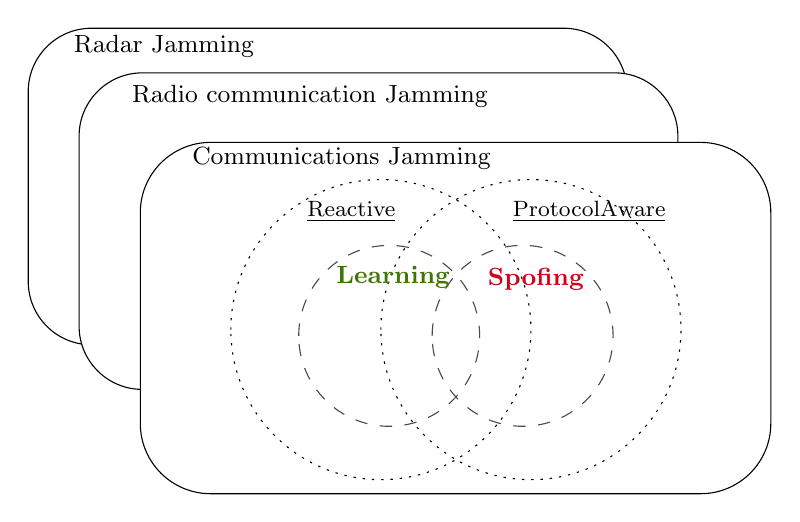
\begin{tikzpicture}[x=0.75pt,y=0.75pt,yscale=-1,xscale=1]
%uncomment if require: \path (0,271); %set diagram left start at 0, and has height of 271

%Rounded Rect [id:dp8149862988479615] 
\draw  [color={rgb, 255:red, 0; green, 0; blue, 0 }  ,draw opacity=1 ][fill={rgb, 255:red, 255; green, 255; blue, 255 }  ,fill opacity=1 ] (240,50.5) .. controls (240,33.66) and (253.66,20) .. (270.5,20) -- (497.99,20) .. controls (514.84,20) and (528.49,33.66) .. (528.49,50.5) -- (528.49,142.01) .. controls (528.49,158.86) and (514.84,172.52) .. (497.99,172.52) -- (270.5,172.52) .. controls (253.66,172.52) and (240,158.86) .. (240,142.01) -- cycle ;
%Rounded Rect [id:dp22268909078842092] 
\draw  [color={rgb, 255:red, 0; green, 0; blue, 0 }  ,draw opacity=1 ][fill={rgb, 255:red, 255; green, 255; blue, 255 }  ,fill opacity=1 ] (264.5,72.01) .. controls (264.5,55.16) and (278.16,41.5) .. (295.01,41.5) -- (522.49,41.5) .. controls (539.34,41.5) and (553,55.16) .. (553,72.01) -- (553,163.52) .. controls (553,180.36) and (539.34,194.02) .. (522.49,194.02) -- (295.01,194.02) .. controls (278.16,194.02) and (264.5,180.36) .. (264.5,163.52) -- cycle ;
%Rounded Rect [id:dp5817415105659758] 
\draw  [color={rgb, 255:red, 0; green, 0; blue, 0 }  ,draw opacity=1 ][fill={rgb, 255:red, 255; green, 255; blue, 255 }  ,fill opacity=1 ] (294,108.85) .. controls (294,90.16) and (309.16,75) .. (327.85,75) -- (563.92,75) .. controls (582.61,75) and (597.77,90.16) .. (597.77,108.85) -- (597.77,210.42) .. controls (597.77,229.12) and (582.61,244.27) .. (563.92,244.27) -- (327.85,244.27) .. controls (309.16,244.27) and (294,229.12) .. (294,210.42) -- cycle ;
%Shape: Circle [id:dp1565825287408389] 
\draw  [color={rgb, 255:red, 0; green, 0; blue, 0 }  ,draw opacity=1 ][dash pattern={on 0.84pt off 2.51pt}] (409.9,165.21) .. controls (409.9,125.28) and (442.27,92.91) .. (482.2,92.91) .. controls (522.12,92.91) and (554.49,125.28) .. (554.49,165.21) .. controls (554.49,205.14) and (522.12,237.5) .. (482.2,237.5) .. controls (442.27,237.5) and (409.9,205.14) .. (409.9,165.21) -- cycle ;
%Shape: Circle [id:dp7239869949598301] 
\draw  [color={rgb, 255:red, 0; green, 0; blue, 0 }  ,draw opacity=1 ][dash pattern={on 0.84pt off 2.51pt}] (337.61,165.21) .. controls (337.61,125.28) and (369.97,92.91) .. (409.9,92.91) .. controls (449.83,92.91) and (482.2,125.28) .. (482.2,165.21) .. controls (482.2,205.14) and (449.83,237.5) .. (409.9,237.5) .. controls (369.97,237.5) and (337.61,205.14) .. (337.61,165.21) -- cycle ;
%Shape: Circle [id:dp6631498600009147] 
\draw  [color={rgb, 255:red, 74; green, 74; blue, 74 }  ,draw opacity=1 ][dash pattern={on 4.5pt off 4.5pt}] (370.32,168.21) .. controls (370.32,144.14) and (389.83,124.62) .. (413.9,124.62) .. controls (437.97,124.62) and (457.49,144.14) .. (457.49,168.21) .. controls (457.49,192.28) and (437.97,211.79) .. (413.9,211.79) .. controls (389.83,211.79) and (370.32,192.28) .. (370.32,168.21) -- cycle ;
%Shape: Circle [id:dp038787615250740703] 
\draw  [color={rgb, 255:red, 74; green, 74; blue, 74 }  ,draw opacity=1 ][dash pattern={on 4.5pt off 4.5pt}] (434.61,168.21) .. controls (434.61,144.14) and (454.13,124.62) .. (478.2,124.62) .. controls (502.27,124.62) and (521.78,144.14) .. (521.78,168.21) .. controls (521.78,192.28) and (502.27,211.79) .. (478.2,211.79) .. controls (454.13,211.79) and (434.61,192.28) .. (434.61,168.21) -- cycle ;

% Text Node
\draw (260.76,22) node [anchor=north west][inner sep=0.75pt]  [font=\small,color={rgb, 255:red, 0; green, 0; blue, 0 }  ,opacity=1 ] [align=left] {Radar Jamming};
% Text Node
\draw (288.76,46) node [anchor=north west][inner sep=0.75pt]  [font=\small,color={rgb, 255:red, 0; green, 0; blue, 0 }  ,opacity=1 ] [align=left] {Radio communication Jamming};
% Text Node
\draw (317.76,76) node [anchor=north west][inner sep=0.75pt]  [font=\small,color={rgb, 255:red, 0; green, 0; blue, 0 }  ,opacity=1 ] [align=left] {Communications Jamming};
% Text Node
\draw (373.25,102.26) node [anchor=north west][inner sep=0.75pt]   [align=left] {{\footnotesize \textcolor[rgb]{0,0,0}{\underline{Reactive}}}};
% Text Node
\draw (472.25,102.26) node [anchor=north west][inner sep=0.75pt]   [align=left] {{\footnotesize \textcolor[rgb]{0,0,0}{\underline{ProtocolAware}}}};
% Text Node
\draw (387.25,133.26) node [anchor=north west][inner sep=0.75pt]  [font=\small] [align=left] {\textcolor[rgb]{0.25,0.46,0.02}{{\small \textbf{Learning}}}};
% Text Node
\draw (460.25,134.26) node [anchor=north west][inner sep=0.75pt]  [font=\small,color={rgb, 255:red, 208; green, 2; blue, 27 }  ,opacity=1 ] [align=left] {\textcolor[rgb]{0.82,0.01,0.11}{{\small \textbf{Spofing}}}};
\end{tikzpicture}
}
\caption{Key capabilities of a jammer and how they relate.} \label{fig:Jammers}
\end{figure}

\begin{itemize}
 \item {In the infinite time space, we are going to build a Machine Learning model which will take as input frequencies by sensing from the wireless network, and try to predict the jammer next action (channel estimation), which literally means that try to determine the next communication channel will jam. And it will allow us to determine the jamming activity pattern in the ad-hoc network, and by analyzing these patterns we are going to concrete  mitigation strategies. So, related research will propose novel techniques to answer the question below,
     
     How to catalyze the jamming activity pattern and initialize effective and relentless mitigation strategies for communication nodes collectively in wireless ad-hoc networks by using autonomous learning techniques ?}
     
 \item {In the first item, we have proposed a method which allows us to analyze the jammer behaviour pattern, and generate defence strategies for the CN based on this pattern. However, in the wireless spectrum we have two different CNs and we can have more nodes, in this case we may transfer the produced policy (or strategy) from one node to another when suitable conditions are satisfied. Moreover, collaborative learning can increase the chances to mitigate against reactive and strong jammers by saving time and energy of CNs. E.g, the cost of learning, cost of transmission, and accuracy of learning models have  high importance roles in the decision model of the framework. 
  
 	Therefore, related research will address the question below, 
 	How the collaborative (transfer) learning can assist knowledge transmission between two different communication nodes in the wireless ad-hoc communication spectrum ? 
 }

 \item{In second item we introduced collective (transfer learning) technique, but when a jamming attack hit the wireless network, there won't be any data transmission in this condition, each CNs have to run their own learning algorithm. } 
\end{itemize}




\chapter{Literature Review}

Numerous anti-jamming methods have been proposed in the literature, ranging from frequency hopping \cite{6117758} \cite{8567751} methods that employ techniques such as honeypots to obtain the jammer policy or to harvest the jamming energy \cite{Bhunia2018CRHoneynetAC} \cite{9149223}. Frequency hopping methods continuously switch the carrier frequency between different bands and can be performed using strategies such as chaotic frequency hopping.

The work in \cite{8664589} proposes a collaborative anti-jamming algorithm (CMAA) in which users collaborate with each other in terms of frequency channel selection in order to mitigate the jammer's effects. 

In \cite{9149223}, the authors propose an spectrum sensing based anti-jamming method where legitimate users mitigate the jamming effects by enhancing their awareness about the jammed channels.

In \cite{8761848}, the authors employ a deep Q-learning learning (DQL) based anti-jamming method to mitigate the effects of a powerful Markov jammer. The work in \cite{Xiao2018ReinforcementLN} proposes a deep reinforcement learning (RL) based anti-jamming technique against a smart jammer in a non- orthogonal multiple access system. In \cite{8314744}, the authors employ deep RL (DRL) to secure the communication between a transmitter and a receiver against multi-jammers. 


The work in \cite{Slimeni2018AMQ} proposes a modified Q-learning technique, where all the Q-values of the Q-table are updated at each iteration, to mitigate the effects of a sweeping jammer. A DRL based method to obtain the optimal task offloading policy under jamming attacks in the context of multi-radio access is pro-posed in \cite{9136780}. Authors in \cite{8792369} propose the idea of harvesting the transmitted power by jammers for data transmission. 

The work \cite{CCRN_Dastangoo_Fossa} in introduces a system consisting of two groups of nodes, namely legitimate users and jammers, that compete to dominate the shared spectrum. In this regard, multi-agent Q-learning is employed to discover the optimal actions of the nodes. 

The works in \cite{8371277} develop anti-jamming methods that employ new approaches to deceive the jammer using a honeypot or fake transmission. 

\cite{9383211} proposed a transfer Game-Actor-Critic (TGACT) scheme, which uses the transferred knowledge in a double-game period to accelerate the learning process and provide performance improvement in channel selection. This work particularly close our research motivation that mentioned this paper, main difference they used other type of RL algorithm rather than deep q-learning algorithm.


In summary, anti-jamming in the practical case of partially observable environment against advanced jammers is an understudied topic in the open technical literature. Thus, in this paper, to ensure safe communication channels for the legitimate users and avoid channel switching, a collaborative autonomous anti-jamming mechanism is proposed by deceiving reactive jammers in partially observable environments, which is applicable to both multi user and single user scenarios. Moreover, we consider the problem of selecting the optimal channel that can be used to deceive the jammer from several available channels.

Specifically based on the state of the system, the long-term network performance is maximized to find the optimal channel policy collectively that can be used against jammer's attack. Moreover Transfer Learning (collaborative learning) technology is accelerate the learning process and to provide performance improvements in channel selection, compared with a classic multi-agent deep reinforcement learning algorithms.




\chapter{Proposed methodologies}

\section{Preliminaries}


\subsection{Fundamentals of Transfer Learning}


Transfer Learning, simply learned knowledge will be transferred from the source domain to the target domain to improve the learning process of the target task. Thus, in the following, we first present the definition of a "domain" and  In our research problem, the source domain is the communication node (CN) that underwent the jammer attack, And the target domain is the likelihood closest unattacked communication node in the wireless network.

\begin{definition}
''Domain: A domain $\displaystyle \mathcal{D}$ is defined by two parts: (i) a feature space $\displaystyle \mathcal{X}$ and (ii) a marginal probability distribution $\displaystyle \mathcal{P}( X)$ in which $\displaystyle X\ =\ \{x_{1,\dotsc ,x_{n}}\} \ \in \ \mathcal{X}$ where $\displaystyle n$ is the number of feature vectors in $\displaystyle \mathcal{X} .$ As such $\displaystyle \mathcal{D} \ =\ \{\mathcal{X} ,\mathcal{P}( X)\}$."
\end{definition}

\begin{definition}
"Task: given domain $\displaystyle \mathcal{D}$, a task $\displaystyle \mathcal{T}$ is defined by two parts: (i) a label space $\displaystyle \mathcal{L}$ and (ii) a predictive function $\displaystyle f( .)$. The predictive function (or decision function) is learned from the feature vector and label space pairs $\displaystyle \{x_{i,\ l_{i}}\}$, with \ $\displaystyle x_{i} \ \in \ X$ and $\displaystyle l_{i} \ \in \ \mathcal{L}$. In other words, a task is defined by $\displaystyle \mathcal{T} \ =\ \{\mathcal{L} ,\ f( .)\}$."
\end{definition}

\begin{definition}
"Transfer Learning: Given a source domain $\displaystyle \mathcal{D}_{S}$ with a corresponding source task \ $\displaystyle \mathcal{T}_{S}$ and a target domain $\displaystyle \mathcal{D}_{T}$ with a corresponding target task $\displaystyle \mathcal{T}_{T}$, the goal of TL is to learn the target predictive function $\displaystyle f_{T}( .)$ by leveraging the knowledge gained from $\displaystyle \mathcal{D}_{S}$ and $\displaystyle \mathcal{T}_{S}$ where $\displaystyle \mathcal{D}_{S} \ \neq \ \mathcal{D}_{T}$ or $\displaystyle \mathcal{T}_{S} \ \neq \ \mathcal{T}_{T}$."
\end{definition}

\subsection{Transfer Learning Techniques}

The key fundamental of TL is utilizing knowledge learned from the source domain to improve the learning of the tar- get domain. To guarantee a good transfer performance, the following three main issues need to be taken into account.

\begin{itemize}
	\item What to transfer: Deciding what will be transferred is the most critical step in TL. To address this issue, one needs to decide which part of learned knowledge will be transferred to improve the learning process of the target domain. This stems from the fact that not all learned knowledge from the source domain will be useful for the target domain in many scenarios. For example, some knowledge can be common in both the source and the target domains, whereas some knowledge is specific to the source domain but not the target domain.
	\item When to transfer: Transferring knowledge is not always helpful in speeding up the learning process of the target domain. Thus, one needs to know when the knowledge should not be transferred. For instance, if the target domain does not have anything in common with the source domain, i.e., they are not related, TL may not improve the learning process and even make the learning process less effective (i.e., negative transfer).
	\item How to transfer: Once the what and when questions have been addressed, one can proceed to transfer learned knowledge to the target domain. This process requires different techniques and designs to maximize the trans- ferring utilization at the target domain.
\end{itemize}


\subsection{Transfer Learning in Deep Reinforcement Learning}

In this section, we first provide fundamental knowledge for DRL and then discuss how TL can be applied to improve the performance of DRL algorithms.

\begin{enumerate}
	\item Deep Reinforcement Learning:
	\begin{enumerate}
		\item {Markov decision process (MDP): MDP is widely used to formulate dynamic decision-making problems. Typically, an MDP is determined by four elements, including a state space $\displaystyle \mathcal{S}$, an action space $\displaystyle \mathcal{A}$, transition probabilities $\displaystyle \mathcal{P}$, i.e., the probability that a state $\displaystyle s_{t}$ at time $\displaystyle t$ moves to state $\displaystyle s_{t+1}$ at time $\displaystyle t\ +1$ after action $\displaystyle a_{t}$ at state $\displaystyle s_{t}$. A mapping from the state space to the action a space is called a policy, denoted by $\displaystyle \pi $. The objective of MDP is usually to find an optimal policy $\displaystyle \pi ^{*}$ that maximizes an expected discounted total reward, i.e., $ $$\displaystyle \pi ^{*} \ =\ \max_{\pi }\mathbb{E}_{\pi }\left[\sum\nolimits ^{T}_{t=0} \gamma ^{t} r_{t}( s_{t} ,\pi ( s_{t}))\right]$ where $\displaystyle a_{t} \ =\ \pi ( s_{t}) ,\mathbb{E}[ .]$ is the expectation function, and $\displaystyle \gamma \ \in \ [ 0,1)$ is the discount factor representing the importance of future rewards.
	 In particular representing the importance of future rewards. In particular, the larger the discount factor is, the more important future rewards are. In practice, due to outstanding abilities to deal with uncertainties in intelligent systems, MDP has been widely adopted to address various problems in dynamic wireless environments, such as spectrum management, cognitive radios, wireless security, and power control. \cite{7080987}}
	 \item {Reinforcement learning (RL): RL is a unique class of ML. An RL agent operates in a dynamic environment formulated by an MDP framework, and its goal is to learn an optimal policy to maximize the expected discounted total reward. During the learning process, the agent interacts with the environment and observes results to gradually find its optimal policy. Specifically, at each time step $\displaystyle t$, the agent observes current state $\displaystyle s_{t}$,

performs action $\displaystyle a_{t}$, according to its current policy, then receives an intermediate reward $\displaystyle r_{t}$ and moves to new  state $\displaystyle s_{t+1}$. After that, the agent adjust its policy based on the feedback of the environment, i.e., $\displaystyle r_{t}$ and $\displaystyle s_{t+1}$.

This procedure us repeated until the agent's policy converges to the optimal one. In practice, Q-learning is one of the most widely used RL algorithms. This algorithm requires evaluating a state- action value function $\displaystyle Q^{\pi }( s,a)$, also called Q-function, that specifies how good of performing an action $\displaystyle a$ at a state $\displaystyle s$ under policy $\displaystyle \pi $. The value of each pair of state and actions is called Q-value. 

The Q-function under the optimal policy $\displaystyle \pi ^{*}$ is called the optimal state-value function $\displaystyle Q^{*}( s,a)$. Suppose that values of $\displaystyle Q^{*}( s,a)$ for all state-action pairs (s,a) are known, the RL agent can obtain the optimal policy at state $\displaystyle s$ by simply taking an action that maximizes $\displaystyle Q^{*}( s,a)$ \cite{Sutton+Barto:1998}. The Q-learning employs a table, namely Q-table, store and update Q-values. Specifically, each cell in the Q-table stores an estimation of the Q-value for each state-action pair. Based on interactions between the agent and the environment at time $\displaystyle t,$ i.e., action $\displaystyle a_{t}$, intermediate reward $\displaystyle r_{t}$, and next state $\displaystyle s_{t+1}$, the Q-function is updated using the temporal difference (TD), which is difference between target Q-value, i.e., $\displaystyle Y_{t} =\ r_{t}( s_{t} ,a_{t}) \ +\ \gamma \max_{a_{t+1}} Q_{t}( s_{t+1} ,a_{t+1}) ,$ and the current estimated Q-value, i.e., $\displaystyle Q_{t}( s_{t} ,a_{s_{t}})$ as follows:
\begin{equation}
Q_{t}( s_{t} ,a_{t}) \ \leftarrow Q_{t}( s_{t} ,a_{t}) \ +\ \zeta _{t}[ Y_{t} -Q_{t}( s_{t,} a_{s_{t}})] .
\end{equation}

where $\displaystyle \zeta _{t}$ is the learning rate that represents the impact of new iteration, i.e., TD. If the Q-function is updated by (3.1) and the learning rate $\displaystyle \zeta _{t}$ satisfies condition in (3.2), it is proven that the policy learn by the Q-learning will converge to the optimal policy. \cite{zhu2021transfer}

\begin{equation}
\zeta _{t} \ \in \ [ 0,1) ,\ \sum ^{\infty }_{t\ =1} \zeta _{t} \ =\ \infty ,\ and\ \sum ^{\infty }_{t\ =1}( \zeta _{t})^{2} \ < \ \infty .
\end{equation}

It is worth nothing that although the convergence of Q-learning is proven, this algorithm is inefficiency in the case of high dimensional state and action spaces since it uses a table for estimating $\displaystyle Q^{*}( s,a)$. Thus, DRL has been introduced recently as a highly-effective solution to address the current limitations of RL algorithms.
}	     	
\item{
Deep reinforcement learning: In a high dimension environment, which has an enormous number of states and actions, the traditional RL methods, e.g., Q-learning, may not handle it effectively. For example, considering the problem of designing an RL-based agent to play various video games without knowing the rules in advance, states can be represented by images consisting of millions of pixels, making it impractical to construct a Q-table. Furthermore, it is inefficient to learn all state-action values in all states separately as that of the Q-learning algorithm. These challenges can be effectively addressed by leveraging DNN architecture for RL algorithms, i.e., DRL. The existing DRL methods can be grouped into value- and policy-based categories.

In the first category, an agent first needs to learn a value function, e.g., the Q-function, then finds the optimal policy based on this function. Most of the value-based DRL methods rely on the Q-learning algorithm, namely Deep Q-learning. Deep Q-learning employs a DNN instead of a Q-table to learn the Q-function

}
	\end{enumerate} 
\end{enumerate}


\subsection{Evaluating Transfer Learning Approaches in DRL}

\begin{itemize}
\item \textbf{What knowledge has been transferred: }Knowledge comes from the source domain and can take different forms of supervisions, such as a set of expert experi- ences, the action probability distribution of an expert policy, or even a potential function that estimates the quality of state and action pairs in the source/target MDP. 
\item \textbf{Where the transfer occurs: }For arbitrary RL task, the MDP (environment) can be defined as a tuple of

$\displaystyle \mathcal{M} \ =\ ( \mu _{0} \ S,\ \mathcal{A} ,\mathcal{T} ,\ \gamma ,\ \mathcal{R} ,\mathcal{S}_{0})$ The source MDP $\displaystyle \mathcal{M}_{s}$ is the place where the prior knowledge comes from and the target MDP $\displaystyle \mathcal{M}_{t}$ is where the knowledge is transferred to. 
\item \textbf{How to transfer knowledge between source and target MPDs:} This question can be rephrased as different sub-questions, such as: What assumptions have been made on the similarity of $\displaystyle \mathcal{M}_{s}$ to $\displaystyle \mathcal{M}_{t}$? Is the mapping function from $\displaystyle \mathcal{M}_{s}$to $\displaystyle \mathcal{M}_{t}$ pre-defined or autonomous generated ? 

What components of the learning procedure, e.g. learning the policy $\displaystyle \pi $, the value function $\displaystyle V$, or even the transition dynamics $\displaystyle \mathcal{T}$ (for model-based RL), can benefit from the transferred knowledge?
\item \textbf{What goal to achieve for the transfer learning approach:} We can answer this question by analyzing two aspect of an TL approach: We can answer this question by analyzing two aspects of an TL approach: (i) its optimization objective function, and (ii) its evaluation metrics. Evalu- ation metrics can be the initial/convergence/episodic performance, or the training iterations/samples used to reach a certain threshold.
\item \textbf{How applicable a TL approach is:} We can rephrase this question as other forms, e.g., Is the TL approach policy-agnostic, or applicable only to certain set of algorithms, e.g, Temporal Difference (TD) methods? Answers to this question are closely related to the form of the transferred knowledge and the similarity between two MDPs.
\item \textbf{What is the accessibility of the target MDP: }We assume that the cost of accessing knowledge from source domains are cheaper. However, the learning agent may not be able to access the target MDP directly, or it can only have a very limited number of MDP interactions, due to the high sampling cost in the target MDP.
\item \textbf{How sample efficient the TL approach is:} This ques- tion is related to the above question regarding the accessibility of a target MDP. Based on the number of interactions needed to enable TL, we can categorize TL techniques into the following classes: (i) Zero-shot transfer: the learned agent are directly applicable to the target MDP without requiring any interactions with it; (ii) Few-shot transfer: only a few samples (interactions) are needed from the target MDP; (iii) Sample-efficient transfer: most of other algorithms fall into this category, where an agent can benefit from TL to learn faster with fewer interactions, which is therefore more sample efficient, compared with a standard RL procedure without any knowledge transfer. Compared with training from scratch in the target MDP, TL approach enable the target agent with a better initial performance and/or converge faster.
\end{itemize}




\section{Problem Statement}




\begin{table}[!h]
        \centering
        
        \parbox{0.65\textwidth}{\caption{Problem notation table}\label{tab:testAp}}
        
\begin{tabular}{|p{0.50\textwidth}|p{0.50\textwidth}|}
\hline 
 Notation & Description \\
\hline 
 $\displaystyle P1$ & Transmit power of the sender communication node \\
\hline 
 $\displaystyle P$2 & Jamming power of the $\displaystyle lth$ jammer \\
\hline 
 R & number of \ transmit power levels \\
\hline 
 I & number of jamming power levels \\
\hline 
 L & number of jammers \\
\hline 
 N  & number of channels \\
\hline 
 $\displaystyle x^{( k)}$ & channel chosen by the sender communication node \\
\hline 
 $\displaystyle y_{l}^{( k)}$ & channel chosen by the $\displaystyle lth$ jammer \\
\hline 
 $\displaystyle h_{s}$ & channel power gain of the sender communication node \\
\hline 
 $\displaystyle h_{l}$ & channel power gain of the $\displaystyle lth\ $ jammer \\
\hline 
 $\displaystyle \gamma $ & discount factor \\
\hline 
 $\displaystyle \pi $ & policy of sender communication node \\
\hline 
 $\displaystyle Q^{source}\left( s^{( k)} ,a^{( k)}\right)$ & Q-function of source domain in time slot k \\
\hline 
 $\displaystyle Q^{target}\left( s^{( k)} ,a^{( k)}\right)$ & Q-function of target domain in time slot k \\
\hline 
 CN & The number of communication nodes. \\
 \hline
\end{tabular}
        
 \end{table}
 
 
 \begin{figure}
 \centering 
	\scalebox{1.0}{
\tikzset{every picture/.style={line width=0.75pt}} %set default line width to 0.75pt        
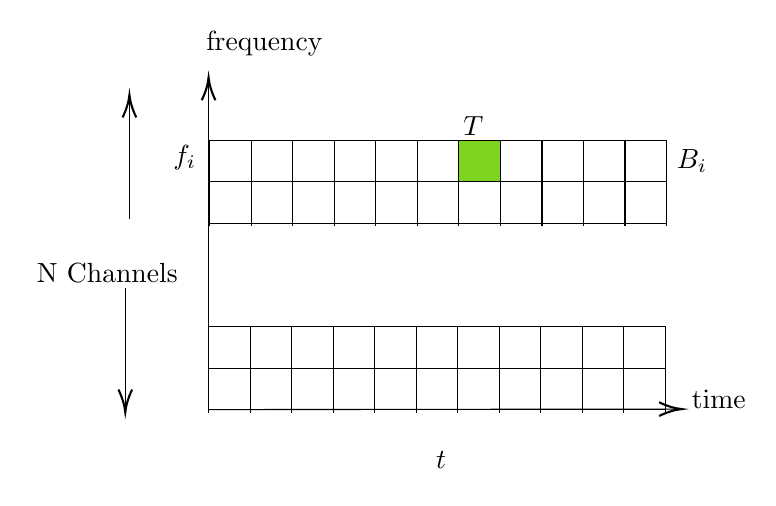
\begin{tikzpicture}[x=0.75pt,y=0.75pt,yscale=-1,xscale=1]
%uncomment if require: \path (0,300); %set diagram left start at 0, and has height of 300

%Straight Lines [id:da7206867047162631] 
\draw    (99.38,232.75) -- (99.38,74.75) ;
\draw [shift={(99.38,72.75)}, rotate = 450] [color={rgb, 255:red, 0; green, 0; blue, 0 }  ][line width=0.75]    (10.93,-3.29) .. controls (6.95,-1.4) and (3.31,-0.3) .. (0,0) .. controls (3.31,0.3) and (6.95,1.4) .. (10.93,3.29)   ;
%Straight Lines [id:da49226471285143525] 
\draw    (99.38,232.75) -- (325.38,232.5) ;
\draw [shift={(327.38,232.5)}, rotate = 539.94] [color={rgb, 255:red, 0; green, 0; blue, 0 }  ][line width=0.75]    (10.93,-3.29) .. controls (6.95,-1.4) and (3.31,-0.3) .. (0,0) .. controls (3.31,0.3) and (6.95,1.4) .. (10.93,3.29)   ;
%Shape: Grid [id:dp8574182637596066] 
\draw  [draw opacity=0] (100,103) -- (320.38,103) -- (320.38,144.5) -- (100,144.5) -- cycle ; \draw   (100,103) -- (100,144.5)(120,103) -- (120,144.5)(140,103) -- (140,144.5)(160,103) -- (160,144.5)(180,103) -- (180,144.5)(200,103) -- (200,144.5)(220,103) -- (220,144.5)(240,103) -- (240,144.5)(260,103) -- (260,144.5)(280,103) -- (280,144.5)(300,103) -- (300,144.5)(320,103) -- (320,144.5) ; \draw   (100,103) -- (320.38,103)(100,123) -- (320.38,123)(100,143) -- (320.38,143) ; \draw    ;
%Shape: Grid [id:dp40455720391260397] 
\draw  [draw opacity=0] (99.38,192.75) -- (319.77,192.75) -- (319.77,234.25) -- (99.38,234.25) -- cycle ; \draw   (99.38,192.75) -- (99.38,234.25)(119.38,192.75) -- (119.38,234.25)(139.38,192.75) -- (139.38,234.25)(159.38,192.75) -- (159.38,234.25)(179.38,192.75) -- (179.38,234.25)(199.38,192.75) -- (199.38,234.25)(219.38,192.75) -- (219.38,234.25)(239.38,192.75) -- (239.38,234.25)(259.38,192.75) -- (259.38,234.25)(279.38,192.75) -- (279.38,234.25)(299.38,192.75) -- (299.38,234.25)(319.38,192.75) -- (319.38,234.25) ; \draw   (99.38,192.75) -- (319.77,192.75)(99.38,212.75) -- (319.77,212.75)(99.38,232.75) -- (319.77,232.75) ; \draw    ;
%Shape: Rectangle [id:dp3287841947190009] 
\draw  [fill={rgb, 255:red, 126; green, 211; blue, 33 }  ,fill opacity=1 ] (220,103) -- (240,103) -- (240,123) -- (220,123) -- cycle ;
%Straight Lines [id:da05175018907140938] 
\draw    (61.25,141.04) -- (61.25,83.04) ;
\draw [shift={(61.25,81.04)}, rotate = 450] [color={rgb, 255:red, 0; green, 0; blue, 0 }  ][line width=0.75]    (10.93,-3.29) .. controls (6.95,-1.4) and (3.31,-0.3) .. (0,0) .. controls (3.31,0.3) and (6.95,1.4) .. (10.93,3.29)   ;
%Straight Lines [id:da7355644094422529] 
\draw    (59.25,174.04) -- (59.25,232.04) ;
\draw [shift={(59.25,234.04)}, rotate = 270] [color={rgb, 255:red, 0; green, 0; blue, 0 }  ][line width=0.75]    (10.93,-3.29) .. controls (6.95,-1.4) and (3.31,-0.3) .. (0,0) .. controls (3.31,0.3) and (6.95,1.4) .. (10.93,3.29)   ;

% Text Node
\draw (97,49) node [anchor=north west][inner sep=0.75pt]   [align=left] {frequency};
% Text Node
\draw (331,222) node [anchor=north west][inner sep=0.75pt]   [align=left] {time};
% Text Node
\draw (96.62,111.39) node   [align=left] {\begin{minipage}[lt]{21.247343750000002pt}\setlength\topsep{0pt}
$\displaystyle f_{i}$
\end{minipage}};
% Text Node
\draw (230.75,96.27) node   [align=left] {\begin{minipage}[lt]{12.920000000000002pt}\setlength\topsep{0pt}
$\displaystyle T$
\end{minipage}};
% Text Node
\draw (332.75,113.02) node   [align=left] {\begin{minipage}[lt]{11.56pt}\setlength\topsep{0pt}
$\displaystyle B_{i}$
\end{minipage}};
% Text Node
\draw (62,167) node   [align=left] {\begin{minipage}[lt]{68pt}\setlength\topsep{0pt}
N Channels
\end{minipage}};
% Text Node
\draw (216.75,257.02) node   [align=left] {\begin{minipage}[lt]{11.56pt}\setlength\topsep{0pt}
$\displaystyle t$
\end{minipage}};
\end{tikzpicture}
}
\caption{Dynamic Spectrum Access (DSA).} \label{fig:DSA}
\end{figure}
 
\begin{table}[h]
        \centering
        
\begin{tabular}{|p{0.25\textwidth}|p{0.19\textwidth}|p{0.20\textwidth}|p{0.20\textwidth}|}
\hline 
 Comm Equipment (CE)  & Jammer & Outcome & Reward \\
\hline 
 Tx & $\displaystyle \emptyset $ & CE Tx Success  &  $\displaystyle R_{CE\ } \ +=\ B$ \\
\hline 
 Tx & Jam & J Jamming & $\displaystyle R_{Jam\ } \ +=\ B$ \\
\hline 
 Tx & Tx & Tx collision & - \\
\hline 
 $\displaystyle \emptyset $ & Jam &  & - \\
 \hline
\end{tabular}
        \caption{Node Actions, outcome and resulting reward}
        \end{table} 
 
\begin{table}[h]

 \centering       
\begin{tabular}{|p{0.10\textwidth}|p{0.04\textwidth}|p{0.04\textwidth}|p{0.04\textwidth}|p{0.04\textwidth}|p{0.05\textwidth}|p{0.05\textwidth}|p{0.04\textwidth}|p{0.04\textwidth}|p{0.04\textwidth}|p{0.05\textwidth}|p{0.30\textwidth}|}
\hline 
 Channel & 1 & 2 & 3 & 4 &  5 & 6 & 7 & 8 & 9 & 10 &  \\
\hline 
  & $\displaystyle \emptyset $ & $\displaystyle \emptyset $ & $\displaystyle \emptyset $ & $\displaystyle \emptyset $ & $\displaystyle \emptyset $ & $\displaystyle \emptyset $ & $\displaystyle \emptyset $ & 1 & 1 & $\displaystyle \emptyset $ & $\displaystyle CE_{1}$ \ Tx \\
\hline 
  & 1 & $\displaystyle \emptyset $ & $\displaystyle \emptyset $ & 1 & $\displaystyle \emptyset $ & $\displaystyle \emptyset $ & $\displaystyle \emptyset $ & $\displaystyle \emptyset $ & $\displaystyle \emptyset $ & $\displaystyle \emptyset $ & CE Tx \\
\hline 
  & $\displaystyle \emptyset $ & $\displaystyle \emptyset $ & 1 & 1 & $\displaystyle \emptyset $ & $\displaystyle \emptyset $ & $\displaystyle \emptyset $ & $\displaystyle \emptyset $ & $\displaystyle \emptyset $ & $\displaystyle \emptyset $ & Jammer \\
\hline 
  & $\displaystyle \emptyset $ & $\displaystyle \emptyset $ & $\displaystyle \emptyset $ & $\displaystyle \emptyset $ & $\displaystyle \emptyset $ & $\displaystyle \emptyset $ & $\displaystyle \emptyset $ & $\displaystyle \emptyset $ & 1 & $\displaystyle \emptyset $ & Jammer \\
 \hline
\end{tabular}
        \caption{Communications Equipment and Jammer CCAdN node Actions}
\end{table}
 
 
 We consider a wireless communication scenario where a sender such as a wireless device \ transmits \ data to the receiver at time slot $\displaystyle k$ with a transmit power $\displaystyle P1_{k}$. while there are L Jammers who can launch jamming attacks by injecting meaningless interference signals denoted as $\displaystyle P2_{k}^{l} \ \in \ \left\{P2_{k}^{1} ,P2_{k}^{2} ,...,P2_{k}^{L}\right\} .$

Each $\displaystyle P2_{k}^{l}$ has $\displaystyle I$ different power levels. 



 The average power $\displaystyle P_{avg}$ should be less than the peak jamming power $\displaystyle P_{max}$. 



$\displaystyle \ \ P_{avg} \ \leq \ P_{max}$ 



In our model, each jammer is assumed to attack only one channel, At time slot $\displaystyle k,$the sender can choose one of N selectable frequency channels for transmitting denoted by $\displaystyle x^{( k)} .$ Meanwhile, $\displaystyle L$ jammers may select their frequency channels (denoted as $\displaystyle \left\{y_{1}^{( k)} ,\ y_{2}^{( k)} ,\dotsc ,y_{L}^{( k)}\right\}$) for jamming. 
  
 $\displaystyle h_{s}$ and $\displaystyle h_{l}$ denote the channel power gains from the sender and the $\displaystyle lth$ jammer to the receiver respectively. 

If \ we denote $\displaystyle \mathbb{x} \ \triangleq \ ( x_{0,} \dotsc ,x_{n} ,\dotsc ,x_{N})$ as a probability vector for being jammed for channels,


In order to resist jamming attack, the sender needs to choose an unblocked channel $\displaystyle x^{( k)}$ and an appropriate transmit power. In general, variable transmit power model is shown to be superior to be the constant transmit power one under the constraint of the same average power. \ After the receiver gets the signal at time slot k, the $\displaystyle SINR( k)$ is calculated by (1) and returned to the sender through the feedback channel. 
 
\begin{equation}
SINR( k) \ =\ \frac{P1h_{s}}{\beta +\sum _{l=1}^{L} P2h_{l} f\left( x^{( k)} \ =\ y_{l}^{( k)}\right)} ,
\end{equation}
 
 where $\displaystyle \beta $ is the receiver noise power, $\displaystyle P2_{k}^{l}$ denotes the jamming power chosen by the $\displaystyle lth$ jammer and $\displaystyle f( \xi )$ is an indicator function that equals 1 if $\displaystyle \xi $ is true and 0 otherwise. If the jammer is completely blocked by the jammers at time slot k, the sender needs to re-transmit the signal \ This will consume extra energy denoted as $\displaystyle C_{m} .$

It is reasonable that the channel is considered to be blocked if the jamming power takes the maximum value $\displaystyle P2_{k}^{L} .$ In order to make a tradeoff between the energy saving and the communication performance, we define the utility $\displaystyle u_{s}^{( k)}$ of the sender by: 
 
\begin{equation}
u_{s}^{( k)} \ =\ SINR( k) \ -\ C_{m} f\left( P2_{k} \ =\ P2_{k}^{L}\right) f\left( x^{( k)} \ =\ y_{l}^{( k)}\right) \ -\ \frac{C_{s} P1_{k}}{P_{s}^{max}}
\end{equation}

where $\displaystyle C_{S}$ and $\displaystyle P_{S}^{\max}$ denote the unit transmission cost and the maximum transmit power respectively. 



\begin{figure}
\centering



\tikzset{every picture/.style={line width=0.75pt}} %set default line width to 0.75pt        

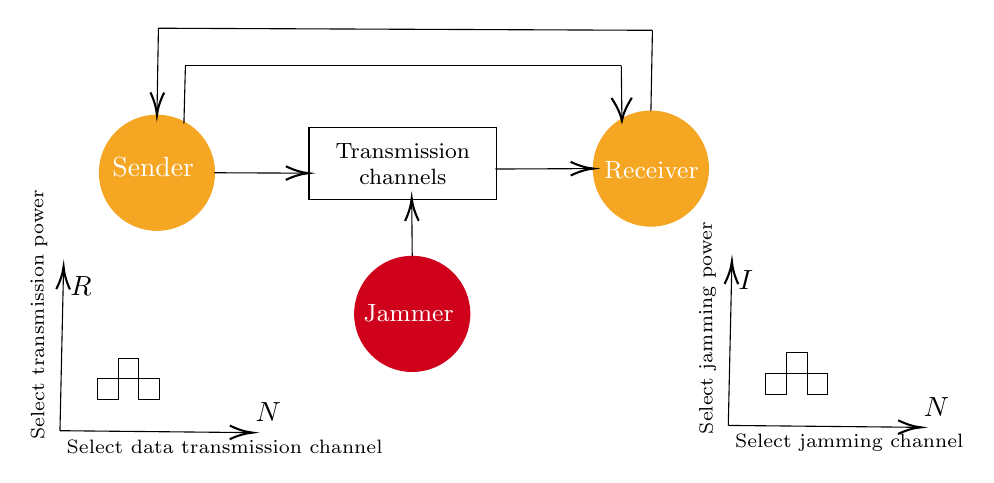
\begin{tikzpicture}[x=0.75pt,y=0.75pt,yscale=-1,xscale=1]
%uncomment if require: \path (0,250); %set diagram left start at 0, and has height of 250

%Shape: Circle [id:dp07282400001791256] 
\draw  [color={rgb, 255:red, 245; green, 166; blue, 35 }  ,draw opacity=1 ][fill={rgb, 255:red, 245; green, 166; blue, 35 }  ,fill opacity=1 ] (195,91.72) .. controls (195,76.41) and (207.41,64) .. (222.72,64) .. controls (238.04,64) and (250.45,76.41) .. (250.45,91.72) .. controls (250.45,107.04) and (238.04,119.45) .. (222.72,119.45) .. controls (207.41,119.45) and (195,107.04) .. (195,91.72) -- cycle ;
%Shape: Circle [id:dp8810702232782299] 
\draw  [color={rgb, 255:red, 245; green, 166; blue, 35 }  ,draw opacity=1 ][fill={rgb, 255:red, 245; green, 166; blue, 35 }  ,fill opacity=1 ] (433,89.72) .. controls (433,74.41) and (445.41,62) .. (460.72,62) .. controls (476.04,62) and (488.45,74.41) .. (488.45,89.72) .. controls (488.45,105.04) and (476.04,117.45) .. (460.72,117.45) .. controls (445.41,117.45) and (433,105.04) .. (433,89.72) -- cycle ;
%Straight Lines [id:da23051797447088207] 
\draw    (223.45,22.09) -- (222.76,62) ;
\draw [shift={(222.72,64)}, rotate = 270.99] [color={rgb, 255:red, 0; green, 0; blue, 0 }  ][line width=0.75]    (10.93,-3.29) .. controls (6.95,-1.4) and (3.31,-0.3) .. (0,0) .. controls (3.31,0.3) and (6.95,1.4) .. (10.93,3.29)   ;
%Straight Lines [id:da07391064886526433] 
\draw    (223.45,22.09) -- (461.45,23.09) ;
%Straight Lines [id:da6338340269715368] 
\draw    (461.45,23.09) -- (460.72,62) ;
%Straight Lines [id:da8445138977081625] 
\draw    (236.45,40.09) -- (235.72,68) ;
%Straight Lines [id:da1164538835183544] 
\draw    (236.45,40.09) -- (446.45,40.09) ;
%Straight Lines [id:da8582506194324306] 
\draw    (446.45,40.09) -- (446.73,64.59) ;
\draw [shift={(446.75,66.59)}, rotate = 269.34000000000003] [color={rgb, 255:red, 0; green, 0; blue, 0 }  ][line width=0.75]    (10.93,-4.9) .. controls (6.95,-2.3) and (3.31,-0.67) .. (0,0) .. controls (3.31,0.67) and (6.95,2.3) .. (10.93,4.9)   ;
%Shape: Rectangle [id:dp742087934688918] 
\draw   (296,70) -- (386.45,70) -- (386.45,104.79) -- (296,104.79) -- cycle ;
%Straight Lines [id:da5253467549833815] 
\draw    (250.45,91.72) -- (293.75,91.92) ;
\draw [shift={(295.75,91.93)}, rotate = 180.26] [color={rgb, 255:red, 0; green, 0; blue, 0 }  ][line width=0.75]    (10.93,-3.29) .. controls (6.95,-1.4) and (3.31,-0.3) .. (0,0) .. controls (3.31,0.3) and (6.95,1.4) .. (10.93,3.29)   ;
%Straight Lines [id:da7112341845701995] 
\draw    (385.75,89.93) -- (431,89.73) ;
\draw [shift={(433,89.72)}, rotate = 539.75] [color={rgb, 255:red, 0; green, 0; blue, 0 }  ][line width=0.75]    (10.93,-3.29) .. controls (6.95,-1.4) and (3.31,-0.3) .. (0,0) .. controls (3.31,0.3) and (6.95,1.4) .. (10.93,3.29)   ;
%Straight Lines [id:da6866335021417969] 
\draw    (176,216) -- (266.75,216.91) ;
\draw [shift={(268.75,216.93)}, rotate = 180.57] [color={rgb, 255:red, 0; green, 0; blue, 0 }  ][line width=0.75]    (10.93,-3.29) .. controls (6.95,-1.4) and (3.31,-0.3) .. (0,0) .. controls (3.31,0.3) and (6.95,1.4) .. (10.93,3.29)   ;
%Straight Lines [id:da8169517027726481] 
\draw    (176,216) -- (177.71,138.93) ;
\draw [shift={(177.75,136.93)}, rotate = 451.27] [color={rgb, 255:red, 0; green, 0; blue, 0 }  ][line width=0.75]    (10.93,-3.29) .. controls (6.95,-1.4) and (3.31,-0.3) .. (0,0) .. controls (3.31,0.3) and (6.95,1.4) .. (10.93,3.29)   ;
%Shape: Rectangle [id:dp22991209794217848] 
\draw   (194,191) -- (204,191) -- (204,201) -- (194,201) -- cycle ;
%Shape: Rectangle [id:dp48508778991210133] 
\draw   (204,181) -- (214,181) -- (214,191) -- (204,191) -- cycle ;
%Shape: Rectangle [id:dp2315856456550467] 
\draw   (214,191) -- (224,191) -- (224,201) -- (214,201) -- cycle ;
%Straight Lines [id:da30711860976564354] 
\draw    (498,213.46) -- (588.75,214.36) ;
\draw [shift={(590.75,214.38)}, rotate = 180.57] [color={rgb, 255:red, 0; green, 0; blue, 0 }  ][line width=0.75]    (10.93,-3.29) .. controls (6.95,-1.4) and (3.31,-0.3) .. (0,0) .. controls (3.31,0.3) and (6.95,1.4) .. (10.93,3.29)   ;
%Straight Lines [id:da57442826910923] 
\draw    (498,213.46) -- (499.71,136.38) ;
\draw [shift={(499.75,134.38)}, rotate = 451.27] [color={rgb, 255:red, 0; green, 0; blue, 0 }  ][line width=0.75]    (10.93,-3.29) .. controls (6.95,-1.4) and (3.31,-0.3) .. (0,0) .. controls (3.31,0.3) and (6.95,1.4) .. (10.93,3.29)   ;
%Shape: Rectangle [id:dp9176657458276827] 
\draw   (516,188.46) -- (526,188.46) -- (526,198.46) -- (516,198.46) -- cycle ;
%Shape: Rectangle [id:dp09230130084447796] 
\draw   (526,178.46) -- (536,178.46) -- (536,188.46) -- (526,188.46) -- cycle ;
%Shape: Rectangle [id:dp8831023123924109] 
\draw   (536,188.46) -- (546,188.46) -- (546,198.46) -- (536,198.46) -- cycle ;
%Shape: Circle [id:dp24118789495729098] 
\draw  [color={rgb, 255:red, 208; green, 2; blue, 27 }  ,draw opacity=1 ][fill={rgb, 255:red, 208; green, 2; blue, 27 }  ,fill opacity=1 ] (318,159.72) .. controls (318,144.41) and (330.41,132) .. (345.72,132) .. controls (361.04,132) and (373.45,144.41) .. (373.45,159.72) .. controls (373.45,175.04) and (361.04,187.45) .. (345.72,187.45) .. controls (330.41,187.45) and (318,175.04) .. (318,159.72) -- cycle ;
%Straight Lines [id:da048994757699609925] 
\draw    (345.72,132) -- (345.49,105.97) ;
\draw [shift={(345.47,103.97)}, rotate = 449.48] [color={rgb, 255:red, 0; green, 0; blue, 0 }  ][line width=0.75]    (10.93,-3.29) .. controls (6.95,-1.4) and (3.31,-0.3) .. (0,0) .. controls (3.31,0.3) and (6.95,1.4) .. (10.93,3.29)   ;

% Text Node
\draw (200,83) node [anchor=north west][inner sep=0.75pt]  [color={rgb, 255:red, 255; green, 255; blue, 255 }  ,opacity=1 ] [align=left] {Sender};
% Text Node
\draw (437,85) node [anchor=north west][inner sep=0.75pt]  [font=\small,color={rgb, 255:red, 255; green, 255; blue, 255 }  ,opacity=1 ] [align=left] {Receiver};
% Text Node
\draw (341.22,87.39) node  [font=\footnotesize] [align=left] {\begin{minipage}[lt]{49.29pt}\setlength\topsep{0pt}
\begin{center}
Transmission\\channels
\end{center}

\end{minipage}};
% Text Node
\draw (269,201.4) node [anchor=north west][inner sep=0.75pt]    {$N$};
% Text Node
\draw (179.75,140.33) node [anchor=north west][inner sep=0.75pt]    {$R$};
% Text Node
\draw (178,219) node [anchor=north west][inner sep=0.75pt]  [font=\scriptsize] [align=left] {Select data transmission channel};
% Text Node
\draw (160.8,221.53) node [anchor=north west][inner sep=0.75pt]  [font=\scriptsize,rotate=-269.71] [align=left] {Select transmission power};
% Text Node
\draw (591,198.86) node [anchor=north west][inner sep=0.75pt]    {$N$};
% Text Node
\draw (501.75,137.78) node [anchor=north west][inner sep=0.75pt]    {$I$};
% Text Node
\draw (500,216.46) node [anchor=north west][inner sep=0.75pt]  [font=\scriptsize] [align=left] {Select jamming channel};
% Text Node
\draw (482.8,218.98) node [anchor=north west][inner sep=0.75pt]  [font=\scriptsize,rotate=-269.71] [align=left] {Select jamming power};
% Text Node
\draw (321,154) node [anchor=north west][inner sep=0.75pt]  [font=\small,color={rgb, 255:red, 255; green, 255; blue, 255 }  ,opacity=1 ] [align=left] {Jammer};
% Text Node
\draw (288.81,77) node [anchor=north west][inner sep=0.75pt]   [align=left] {};

\end{tikzpicture}
\caption{Anti-jamming wireless communication system}\label{fig:AJWC}
\end{figure}

$\displaystyle s^{( k)} \ =\ SINR( k-1) ,$ the system state at time slot k, which is the value of SINR at time slot $\displaystyle k-1$.

$\displaystyle a^{( k)} \ =\ \left[ x^{( k)} ,P1_{k}\right]$, represents the action of sender at time slot k, which contains a frequency channel $\displaystyle x^{( k)}$ and a transmit power $\displaystyle P1_{k}$. After the action is performed, the sender receives a reward $\displaystyle u_{s}^{( k)}$.

\textbf{Q-function:}

\begin{equation}
Q\left( s^{( k)} ,a^{( k)}\right) \ =\ \mathbb{E}\left[ u_{s}^{( k)} \ +\ \gamma \ \underset{a"\ \in A}{\max} Q\left( s^{( k+1)} ,\ a^{'}\right) \ |\ s^{( k)} ,a^{( k)}\right] ,
\end{equation}

Parameters of $\displaystyle \epsilon -greedy$ algorithm: 

$\displaystyle \tau $: represent the probability of performing the previous action $\displaystyle a^{( k-1)}$ directly at time slot k without calculating Q-value.

\begin{equation}
( \tau -\epsilon ) -greedy\ \Longrightarrow \ \pi \left( a^{( k)} |\ s^{( k)}\right) \ =\ \begin{cases}
a^{( k-1)} & with\ probability\ of\ \tau \\
a_{\tau } & with\ probability\ of\ \epsilon \\
\underset{a^{'} \ \in \ A}{\arg\max \ } Q\left( s^{( k)} ,a^{'}\right) & with\ probability\ of\ ( 1-\tau -\epsilon )
\end{cases}
\end{equation}


\begin{equation}
\overline{u}_{s}^{( k-1)} \ \ =\ \frac{1}{T}\sum\nolimits _{i=1}^{T} u_{s}^{( k-i)}
\end{equation}

(3.7) : For the valuable action judgment, we compute the average utility of T previous time slots as a threshold.


\begin{figure}

\centering
\tikzset{every picture/.style={line width=0.75pt}} %set default line width to 0.75pt        

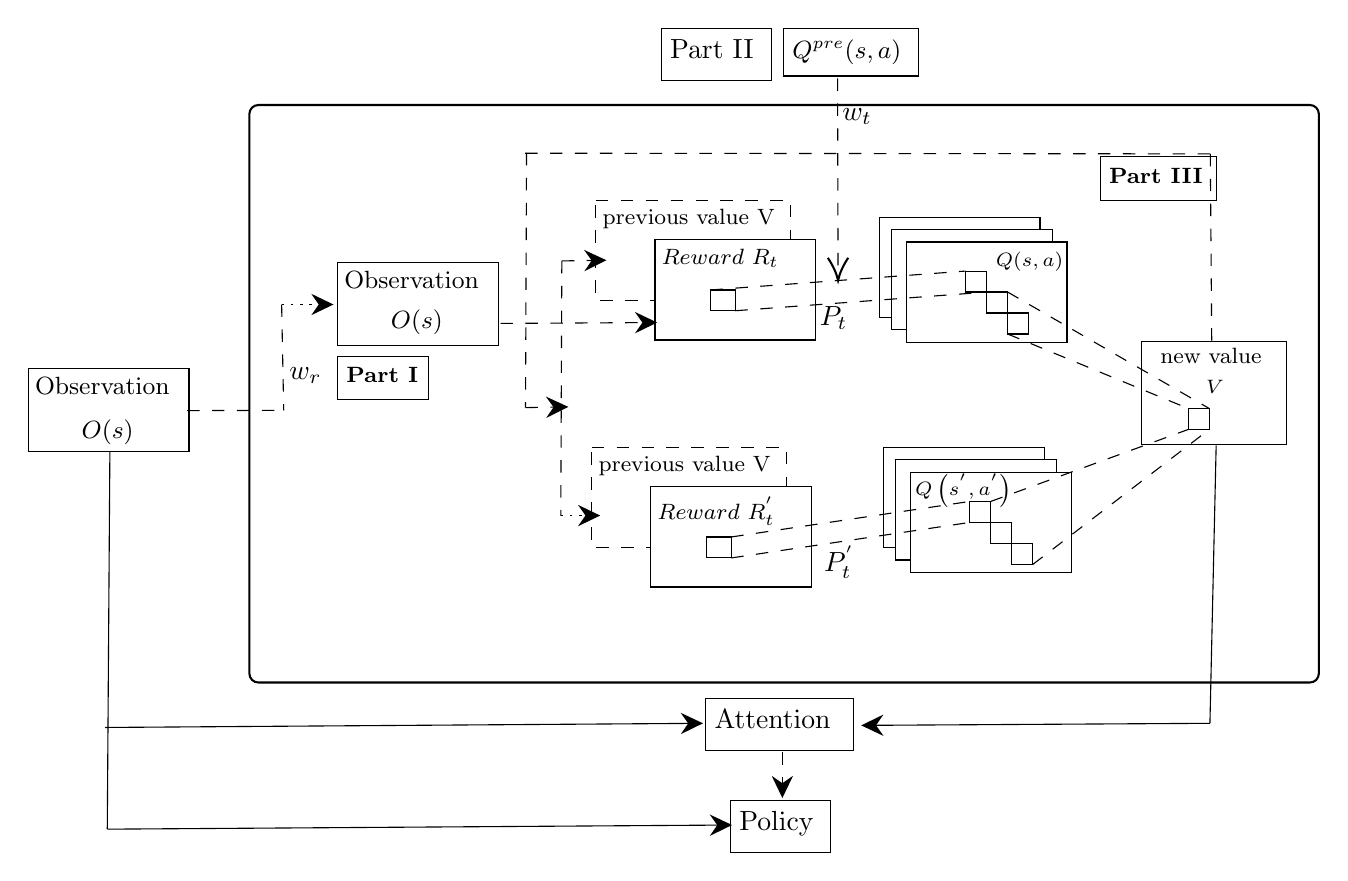
\begin{tikzpicture}[x=0.75pt,y=0.75pt,yscale=-1,xscale=1]
%uncomment if require: \path (0,413); %set diagram left start at 0, and has height of 413

%Rounded Rect [id:dp037038531697400234] 
\draw  [color={rgb, 255:red, 0; green, 0; blue, 0 }  ,draw opacity=1 ][line width=0.75]  (126.74,46.32) .. controls (126.74,43.93) and (128.68,42) .. (131.06,42) -- (637.68,42) .. controls (640.07,42) and (642,43.93) .. (642,46.32) -- (642,315.9) .. controls (642,318.28) and (640.07,320.22) .. (637.68,320.22) -- (131.06,320.22) .. controls (128.68,320.22) and (126.74,318.28) .. (126.74,315.9) -- cycle ;
%Shape: Rectangle [id:dp9112105868230191] 
\draw  [color={rgb, 255:red, 0; green, 0; blue, 0 }  ,draw opacity=1 ] (169.19,118) -- (246.66,118) -- (246.66,158) -- (169.19,158) -- cycle ;
%Shape: Rectangle [id:dp41556728500124507] 
\draw  [color={rgb, 255:red, 0; green, 0; blue, 0 }  ,draw opacity=1 ][fill={rgb, 255:red, 255; green, 255; blue, 255 }  ,fill opacity=1 ] (20.19,169) -- (97.66,169) -- (97.66,209) -- (20.19,209) -- cycle ;
%Straight Lines [id:da31075089348460994] 
\draw  [dash pattern={on 4.5pt off 4.5pt}]  (96.74,189.22) -- (143.28,189.11) ;
%Straight Lines [id:da9289566830128999] 
\draw  [dash pattern={on 4.5pt off 4.5pt}]  (142.28,138.11) -- (143.28,189.11) ;
%Straight Lines [id:da14211003468762828] 
\draw  [dash pattern={on 0.84pt off 2.51pt}]  (142.28,138.11) -- (164.28,138.11) ;
\draw [shift={(167.28,138.11)}, rotate = 180] [fill={rgb, 255:red, 0; green, 0; blue, 0 }  ][line width=0.08]  [draw opacity=0] (10.72,-5.15) -- (0,0) -- (10.72,5.15) -- (7.12,0) -- cycle    ;
%Shape: Rectangle [id:dp8432056909787771] 
\draw  [color={rgb, 255:red, 0; green, 0; blue, 0 }  ,draw opacity=1 ][dash pattern={on 4.5pt off 4.5pt}] (293.69,88) -- (387.66,88) -- (387.66,136.22) -- (293.69,136.22) -- cycle ;
%Shape: Rectangle [id:dp4838012428553906] 
\draw  [color={rgb, 255:red, 0; green, 0; blue, 0 }  ,draw opacity=1 ][fill={rgb, 255:red, 255; green, 255; blue, 255 }  ,fill opacity=1 ] (322.19,107) -- (399.66,107) -- (399.66,155.22) -- (322.19,155.22) -- cycle ;
%Shape: Rectangle [id:dp04392721967580826] 
\draw  [color={rgb, 255:red, 0; green, 0; blue, 0 }  ,draw opacity=1 ][dash pattern={on 4.5pt off 4.5pt}] (291.69,207) -- (385.66,207) -- (385.66,255.22) -- (291.69,255.22) -- cycle ;
%Shape: Rectangle [id:dp08474048927820488] 
\draw  [color={rgb, 255:red, 0; green, 0; blue, 0 }  ,draw opacity=1 ][fill={rgb, 255:red, 255; green, 255; blue, 255 }  ,fill opacity=1 ] (320.19,226) -- (397.66,226) -- (397.66,274.22) -- (320.19,274.22) -- cycle ;
%Shape: Rectangle [id:dp8819293523060772] 
\draw   (348.95,131.11) -- (360.92,131.11) -- (360.92,141.11) -- (348.95,141.11) -- cycle ;
%Straight Lines [id:da9436173005905717] 
\draw  [dash pattern={on 4.5pt off 4.5pt}]  (247.74,147.22) -- (320.22,146.81) ;
\draw [shift={(323.22,146.79)}, rotate = 539.6800000000001] [fill={rgb, 255:red, 0; green, 0; blue, 0 }  ][line width=0.08]  [draw opacity=0] (10.72,-5.15) -- (0,0) -- (10.72,5.15) -- (7.12,0) -- cycle    ;
%Straight Lines [id:da22843514245680185] 
\draw  [dash pattern={on 4.5pt off 4.5pt}]  (277.28,117.11) -- (276.78,239.79) ;
%Straight Lines [id:da3208905432721849] 
\draw  [dash pattern={on 4.5pt off 4.5pt}]  (277.28,117.11) -- (295.78,116.83) ;
\draw [shift={(298.78,116.79)}, rotate = 539.15] [fill={rgb, 255:red, 0; green, 0; blue, 0 }  ][line width=0.08]  [draw opacity=0] (10.72,-5.15) -- (0,0) -- (10.72,5.15) -- (7.12,0) -- cycle    ;
%Straight Lines [id:da8748720532603396] 
\draw  [dash pattern={on 0.84pt off 2.51pt}]  (276.78,239.79) -- (292.78,239.79) ;
\draw [shift={(295.78,239.79)}, rotate = 180] [fill={rgb, 255:red, 0; green, 0; blue, 0 }  ][line width=0.08]  [draw opacity=0] (10.72,-5.15) -- (0,0) -- (10.72,5.15) -- (7.12,0) -- cycle    ;
%Shape: Rectangle [id:dp4584883217062876] 
\draw   (346.95,250.11) -- (358.92,250.11) -- (358.92,260.11) -- (346.95,260.11) -- cycle ;
%Shape: Rectangle [id:dp02643814237674791] 
\draw  [color={rgb, 255:red, 0; green, 0; blue, 0 }  ,draw opacity=1 ][fill={rgb, 255:red, 255; green, 255; blue, 255 }  ,fill opacity=1 ] (430.19,96) -- (507.66,96) -- (507.66,144.22) -- (430.19,144.22) -- cycle ;
%Shape: Rectangle [id:dp5045809733341071] 
\draw  [color={rgb, 255:red, 0; green, 0; blue, 0 }  ,draw opacity=1 ][fill={rgb, 255:red, 255; green, 255; blue, 255 }  ,fill opacity=1 ] (436.19,102) -- (513.66,102) -- (513.66,150.22) -- (436.19,150.22) -- cycle ;
%Shape: Rectangle [id:dp34948397730346614] 
\draw  [color={rgb, 255:red, 0; green, 0; blue, 0 }  ,draw opacity=1 ][fill={rgb, 255:red, 255; green, 255; blue, 255 }  ,fill opacity=1 ] (443.19,108) -- (520.66,108) -- (520.66,156.22) -- (443.19,156.22) -- cycle ;
%Shape: Rectangle [id:dp16704931791016153] 
\draw   (471.78,122) -- (481.92,122) -- (481.92,132.11) -- (471.78,132.11) -- cycle ;
%Shape: Rectangle [id:dp7662910853092366] 
\draw   (481.92,132.11) -- (492.07,132.11) -- (492.07,142.22) -- (481.92,142.22) -- cycle ;
%Shape: Rectangle [id:dp508539462381391] 
\draw   (492.07,142.22) -- (502.21,142.22) -- (502.21,152.32) -- (492.07,152.32) -- cycle ;
%Shape: Rectangle [id:dp7581611272622251] 
\draw  [color={rgb, 255:red, 0; green, 0; blue, 0 }  ,draw opacity=1 ][fill={rgb, 255:red, 255; green, 255; blue, 255 }  ,fill opacity=1 ] (432.19,207) -- (509.66,207) -- (509.66,255.22) -- (432.19,255.22) -- cycle ;
%Shape: Rectangle [id:dp15409364731756714] 
\draw  [color={rgb, 255:red, 0; green, 0; blue, 0 }  ,draw opacity=1 ][fill={rgb, 255:red, 255; green, 255; blue, 255 }  ,fill opacity=1 ] (438.19,213) -- (515.66,213) -- (515.66,261.22) -- (438.19,261.22) -- cycle ;
%Shape: Rectangle [id:dp7087685242693063] 
\draw  [color={rgb, 255:red, 0; green, 0; blue, 0 }  ,draw opacity=1 ][fill={rgb, 255:red, 255; green, 255; blue, 255 }  ,fill opacity=1 ] (445.19,219) -- (522.66,219) -- (522.66,267.22) -- (445.19,267.22) -- cycle ;
%Shape: Rectangle [id:dp979918051905466] 
\draw   (473.78,233) -- (483.92,233) -- (483.92,243.11) -- (473.78,243.11) -- cycle ;
%Shape: Rectangle [id:dp5914386328123566] 
\draw   (483.92,243.11) -- (494.07,243.11) -- (494.07,253.22) -- (483.92,253.22) -- cycle ;
%Shape: Rectangle [id:dp9706407290808747] 
\draw   (494.07,253.22) -- (504.21,253.22) -- (504.21,263.32) -- (494.07,263.32) -- cycle ;
%Straight Lines [id:da7393749883378757] 
\draw  [dash pattern={on 4.5pt off 4.5pt}]  (348.95,131.11) -- (471.78,122) ;
%Straight Lines [id:da40988505368090555] 
\draw  [dash pattern={on 4.5pt off 4.5pt}]  (360.92,141.11) -- (483.76,132) ;
%Straight Lines [id:da396651554718344] 
\draw  [dash pattern={on 4.5pt off 4.5pt}]  (358.92,250.11) -- (473.78,233) ;
%Straight Lines [id:da3634509196932123] 
\draw  [dash pattern={on 4.5pt off 4.5pt}]  (358.92,260.22) -- (473.78,243.11) ;
%Shape: Rectangle [id:dp7284256745819491] 
\draw   (556.4,156) -- (626.4,156) -- (626.4,205.42) -- (556.4,205.42) -- cycle ;
%Shape: Rectangle [id:dp04905544181336596] 
\draw   (579.07,188.22) -- (589.21,188.22) -- (589.21,198.32) -- (579.07,198.32) -- cycle ;
%Straight Lines [id:da23637943461666389] 
\draw  [dash pattern={on 4.5pt off 4.5pt}]  (492.07,132.11) -- (589.21,188.22) ;
%Straight Lines [id:da7471801026142995] 
\draw  [dash pattern={on 4.5pt off 4.5pt}]  (492.07,152.32) -- (579.07,188.22) ;
%Straight Lines [id:da43005278974589234] 
\draw  [dash pattern={on 4.5pt off 4.5pt}]  (483.92,233) -- (579.07,198.32) ;
%Straight Lines [id:da5027402928007583] 
\draw  [dash pattern={on 4.5pt off 4.5pt}]  (504.21,263.32) -- (589.21,198.32) ;
%Straight Lines [id:da5279990177924845] 
\draw  [dash pattern={on 4.5pt off 4.5pt}]  (260.28,65.11) -- (259.78,187.79) ;
%Straight Lines [id:da8561019614280772] 
\draw  [dash pattern={on 4.5pt off 4.5pt}]  (259.59,65.22) -- (589.71,65.54) ;
%Straight Lines [id:da31744004531817915] 
\draw  [dash pattern={on 4.5pt off 4.5pt}]  (589.71,65.54) -- (590.4,156.42) ;
%Straight Lines [id:da3165560078922094] 
\draw  [dash pattern={on 4.5pt off 4.5pt}]  (259.78,187.79) -- (277.4,187.48) ;
\draw [shift={(280.4,187.42)}, rotate = 538.98] [fill={rgb, 255:red, 0; green, 0; blue, 0 }  ][line width=0.08]  [draw opacity=0] (10.72,-5.15) -- (0,0) -- (10.72,5.15) -- (7.12,0) -- cycle    ;
%Straight Lines [id:da7721829350838407] 
\draw  [dash pattern={on 4.5pt off 4.5pt}]  (410.14,29.2) -- (410.36,124.55) ;
\draw [shift={(410.37,126.55)}, rotate = 269.87] [color={rgb, 255:red, 0; green, 0; blue, 0 }  ][line width=0.75]    (10.93,-4.9) .. controls (6.95,-2.3) and (3.31,-0.67) .. (0,0) .. controls (3.31,0.67) and (6.95,2.3) .. (10.93,4.9)   ;
%Straight Lines [id:da7341588320312835] 
\draw  [dash pattern={on 4.5pt off 4.5pt}]  (383.53,353.89) -- (383.53,372.89) ;
\draw [shift={(383.53,375.89)}, rotate = 270] [fill={rgb, 255:red, 0; green, 0; blue, 0 }  ][line width=0.08]  [draw opacity=0] (10.72,-5.15) -- (0,0) -- (10.72,5.15) -- (7.12,0) -- cycle    ;
%Straight Lines [id:da6460991037007136] 
\draw    (592.53,206) -- (589.53,339.89) ;
%Straight Lines [id:da1432138213901859] 
\draw    (589.53,339.89) -- (424.53,340.87) ;
\draw [shift={(421.53,340.89)}, rotate = 359.65999999999997] [fill={rgb, 255:red, 0; green, 0; blue, 0 }  ][line width=0.08]  [draw opacity=0] (10.72,-5.15) -- (0,0) -- (10.72,5.15) -- (7.12,0) -- cycle    ;
%Straight Lines [id:da06654670219633685] 
\draw    (59.53,209) -- (58.28,390.89) ;
%Straight Lines [id:da769957476106125] 
\draw    (57.28,341.89) -- (342.28,339.91) ;
\draw [shift={(345.28,339.89)}, rotate = 539.6] [fill={rgb, 255:red, 0; green, 0; blue, 0 }  ][line width=0.08]  [draw opacity=0] (10.72,-5.15) -- (0,0) -- (10.72,5.15) -- (7.12,0) -- cycle    ;
%Straight Lines [id:da38456746776594897] 
\draw    (58.28,390.89) -- (356.28,388.91) ;
\draw [shift={(359.28,388.89)}, rotate = 539.62] [fill={rgb, 255:red, 0; green, 0; blue, 0 }  ][line width=0.08]  [draw opacity=0] (10.72,-5.15) -- (0,0) -- (10.72,5.15) -- (7.12,0) -- cycle    ;

% Text Node
\draw (171.19,121) node [anchor=north west][inner sep=0.75pt]   [align=left] {{\small \textcolor[rgb]{0,0,0}{Observation}}};
% Text Node
\draw (193.66,139.4) node [anchor=north west][inner sep=0.75pt]  [font=\small]  {$\textcolor[rgb]{0,0,0}{O}\textcolor[rgb]{0,0,0}{(}\textcolor[rgb]{0,0,0}{s}\textcolor[rgb]{0,0,0}{)}$};
% Text Node
\draw (22.19,172) node [anchor=north west][inner sep=0.75pt]   [align=left] {{\small \textcolor[rgb]{0,0,0}{Observation}}};
% Text Node
\draw (44.66,192.4) node [anchor=north west][inner sep=0.75pt]  [font=\small]  {$\textcolor[rgb]{0,0,0}{O}\textcolor[rgb]{0,0,0}{(}\textcolor[rgb]{0,0,0}{s}\textcolor[rgb]{0,0,0}{)}$};
% Text Node
\draw (324.19,110.4) node [anchor=north west][inner sep=0.75pt]  [font=\footnotesize]  {$Reward\ R_{t}$};
% Text Node
\draw (295.69,91) node [anchor=north west][inner sep=0.75pt]  [font=\footnotesize] [align=left] {previous value V};
% Text Node
\draw (322.19,229.4) node [anchor=north west][inner sep=0.75pt]  [font=\footnotesize]  {$Reward\ R_{t}^{'}$};
% Text Node
\draw (293.69,210) node [anchor=north west][inner sep=0.75pt]  [font=\footnotesize] [align=left] {previous value V};
% Text Node
\draw (485.09,111.4) node [anchor=north west][inner sep=0.75pt]  [font=\scriptsize]  {$Q( s,a)$};
% Text Node
\draw (446.19,218.4) node [anchor=north west][inner sep=0.75pt]  [font=\scriptsize]  {$Q\left( s^{'} ,a^{'}\right)$};
% Text Node
\draw (400.37,137.95) node [anchor=north west][inner sep=0.75pt]    {$P_{t}$};
% Text Node
\draw (402.37,252.95) node [anchor=north west][inner sep=0.75pt]    {$P_{t}^{'}$};
% Text Node
\draw (564.4,158) node [anchor=north west][inner sep=0.75pt]  [font=\footnotesize] [align=left] {new value};
% Text Node
\draw (586.4,173.4) node [anchor=north west][inner sep=0.75pt]  [font=\scriptsize]  {$V$};
% Text Node
\draw    (536.65,67) -- (592.65,67) -- (592.65,88) -- (536.65,88) -- cycle  ;
\draw (539.65,71) node [anchor=north west][inner sep=0.75pt]  [font=\footnotesize,color={rgb, 255:red, 0; green, 0; blue, 0 }  ,opacity=1 ] [align=left] {\textbf{Part III}};
% Text Node
\draw    (384.14,5) -- (449.14,5) -- (449.14,28) -- (384.14,28) -- cycle  ;
\draw (387.14,9.4) node [anchor=north west][inner sep=0.75pt]  [font=\small]  {$Q^{pre}( s,a)$};
% Text Node
\draw    (325.14,5) -- (378.14,5) -- (378.14,30) -- (325.14,30) -- cycle  ;
\draw (328.14,9) node [anchor=north west][inner sep=0.75pt]   [align=left] {Part II};
% Text Node
\draw (144.78,167.01) node [anchor=north west][inner sep=0.75pt]    {$w_{r}$};
% Text Node
\draw    (169.25,163) -- (213.25,163) -- (213.25,184) -- (169.25,184) -- cycle  ;
\draw (172.25,167) node [anchor=north west][inner sep=0.75pt]  [font=\footnotesize] [align=left] {\textbf{Part I}};
% Text Node
\draw (411.14,42.6) node [anchor=north west][inner sep=0.75pt]    {$w_{t}$};
% Text Node
\draw    (346.59,328) -- (417.59,328) -- (417.59,353) -- (346.59,353) -- cycle  ;
\draw (349.59,332) node [anchor=north west][inner sep=0.75pt]   [align=left] {Attention};
% Text Node
\draw    (358.53,377) -- (406.53,377) -- (406.53,402) -- (358.53,402) -- cycle  ;
\draw (361.53,381) node [anchor=north west][inner sep=0.75pt]   [align=left] {Policy};
\end{tikzpicture}
\caption{The Framework of TVIN}
\end{figure}

M is represent the MDP of some communication nodes, where an optimal policy $\displaystyle \pi $ is expected to be learned.

The states, actions, rewards and transitions in M are denoted by;
\begin{itemize}
\item $\displaystyle s\ \in \mathcal{\ } S$
\item $\displaystyle a\ \in \mathcal{A}$
\item $\displaystyle R( s,a)$
\item $\displaystyle P\left( s^{'} |s,a\right)$ respectively.
\end{itemize}

$\displaystyle \phi ( s)$ represent an observation for state s.

$\displaystyle \theta $ denotes all the parameters of the Transfer Value Iteration Networks (TVIN)

R and P are dependent on the observations as follows; 
\begin{itemize}
\item $\displaystyle R\ =\ f_{R}( \phi ( s))$
\item $\displaystyle P\ =\ f_{P}( \phi ( s))$
\end{itemize}

The functions $\displaystyle f_{R}$ and $\displaystyle f_{P}$ are learned jointly in the policy learning process.

Given a trained MDP in source communication domain (node), we aim to transfer the learned knowledge including the learned reward function and transition function to the target communication domain (node), such that an optimal policy $\displaystyle \pi ( a|\ \phi ( s) ;\theta )$ for the target domain can be learned. 

Given the trained VIN in the source domain, the trained reward function $\displaystyle f_{R}$ is first transferred to produce reward images for the observations s in the target communication domain.

After that the state transition values on the common subset of actions, $\displaystyle f_{P}^{pre}$, is transferred to the target domain with a learnable weight associated with each action to measure the similarity degree between communication domains. And the state transition values on new domain-specific actions, $\displaystyle f_{P}^{new}$, are learned from scratch.

All these state transition values reconstruct a transition function in the target communication domain, which is further used to compute the Q-function in each iteration for the target communication domain.

An attention vector is fed as \ an input to generate target policy $\displaystyle \pi _{T}$. 

\textbf{Transition function transferring:}

To transfer the transition function across domains, we use value iteration by approximating the Bellman-update through a CNN in the target domain. Specifically, the CNN used for comprised of stacked convolution and max-pooling layers.


The input to each convolution layer is a 3-dimensional signal X, typically, and image with $\displaystyle l$ channels and $\displaystyle m\ \times \ n$ pixels. 

Its output $\displaystyle h$ is a $\displaystyle l'$-channel convolution of the image with different kernels:

\begin{equation*}
h_{l',i',j'} \ =\ \sigma \left(\sum\nolimits _{l,i,j} W_{l,i,j}^{l^{'}} X_{l.i^{'}} -i,j^{'} -j\right)
\end{equation*}
where $\displaystyle \sigma $ is an activation function A max-pooling layer then down-samples the image by selecting the maximum value among some dimension.

\textbf{Problem Formulation:}

\begin{gather}
\underset{s}{\max} \ \sum _{i=1}^{CN}\sum\nolimits _{i=1}^{T} u_{s_{i}}^{( i)}\\
 \notag\\
.s.t.\begin{cases}
\sum\nolimits _{n=0}^{N} x_{n} =0, & \\
x_{n} \ \in \ [ 0,1] ,\ \forall n\ \in \ \{0,\dotsc ,N\} , & \\
\mathbb{x} P2^{T} \ \leq \ P_{avg} & 
\end{cases} \notag
\end{gather}



%\begin{algorithm}[!h]
%
%\caption{Algorithm example}
%
%\KwIn{Gallery with initial templates $\mathcal G = \{\textbf{r}_1,...,\textbf{r}_J\}$, unlabeled adaptation set $\mathcal D = \{\textbf{d}_{1},...,\textbf{d}_{L}\}$}
%\KwOut{Updated Gallery $\mathcal G' = \{\textbf{r}_1,...,\textbf{r}_{J'}\}$, $J' \geq J$}
%\BlankLine
%\BlankLine
%
%Estimate updating threshold $\gamma^u \geq \gamma^d$ from $\mathcal G$\;
%
%$\mathcal G \leftarrow \mathcal G'$\tcc*{update gallery}
%
%	\For{all samples $d_l \in \mathcal D$ ($l=1,...,L$)}{
%		\For{all references $r_j \in \mathcal G$ ($j=1,...,J$)}{
%			$s_j(\textbf{d}_l) \leftarrow similarity\_measure(\textbf{d}_l,\textbf{r}_j)$\;
%		}
%	}
%	
%	$S(\textbf{d}_l) \leftarrow \max\limits_{j \in [1,J]}\{s_j(\textbf{d}_l)\}$\;
%	
%	\If{$S(\textbf{d}_l) \geq \gamma_d$}{
%		Output positive prediction\;
%		
%		\If{$S(\textbf{d}_l)\geq \gamma^u$}{
%			$\mathcal{G'} \leftarrow \mathcal{G'} \cup \textbf{d}_l$\;
%		}
%		
%	}
%\end{algorithm}


\chapter{Preliminary Results}

%%- Conclusion -%%
\begin{conclusion}

\end{conclusion}


%%%%%%%%%%%%%%%%%%%%%%%%%%%%%%%%%%%%%%%%%%%%%%%%%%%
%  Appendix example:
%%%%%%%%%%%%%%%%%%%%%%%%%%%%%%%%%%%%%%%%%%%%%%%%%%%
\appendix

%% To use more than one appendix
\multiannexe

%% Appendix from an external file
% \include{extApp}

\chapter{Appendix}


%%%%%%%%%%%%%%%%%%%%%%%%%%%%%%%%%%%%%%%%%%%%%%%%%%%
% BIBLIOGRAPHY AND REFERENCES
%%%%%%%%%%%%%%%%%%%%%%%%%%%%%%%%%%%%%%%%%%%%%%%%%%%

%%- Bibliography -%%
\newpage
% Single spacing for the bibliography
\begin{spacing}{1}
    \setlength{\bibsep}{\baselineskip}
	\nocite{*} % The "nocite" command can be used to print references that haven't been used in the document. The "*" option specifies that every reference should be printed
	\bibliographystyle{bibETS} % ETS bibliography style
	\addcontentsline{toc}{chapter}{BIBLIOGRAPHY} % Addition of the bibliography in the table of contents

	\bibliography{biblio_en} % List of bibliography files, biblio.bib is an example

\end{spacing}

%%- Other list of references, "refs" example --%
%%%%%%%%%%%%%%%%%%%%%%%%%%%%%%%%%%%%%%%%%%%%%%%%%%%
% IMPORTANT: HOW TO COMPILE AND PRINT ADDITIONAL REFERENCES (replace "refs" by the chosen name)
%%%%%%%%%%%%%%%%%%%%%%%%%%%%%%%%%%%%%%%%%%%%%%%%%%%
% Follow these three steps:
%   1. Compile the document once, to save the used references in refs.aux
%   2. Compile the references
% 		- On Linux: Use the "bibtex refs" command in the document folder
%		- On MacOSX (MacTex distribution): Use the "/usr/texbin/bibtex refs" command in the document folder
%		- On Windows: Edit the "update_refs.bat" script to put the right suffix ("refs" here), and launch the script
%   3. Recompile the document TWICE
%%%%%%%%%%%%%%%%%%%%%%%%%%%%%%%%%%%%%%%%%%%%%%%%%%%

\newpage
% Same commands than for the bibliography, only with the "refs" suffix
\begin{spacing}{1}
    \setlength{\bibsep}{\baselineskip}
	%\nociterefs{*}
	\bibliographystylerefs{bibETS}
	\addcontentsline{toc}{chapter}{LIST OF REFERENCES}

	\bibliographyrefs{refs}

\end{spacing}

\end{document}